\chapter{Test des Systems}
\label{chapter:testing}

	Das Testen dieses Softwaresystem wurde in drei Aufgabenbereiche unterteilt.
	Zuerst wurde das Frontend durchgängig getestet.
	Anschließend wurde das Backend überprüft.
	Letztendlich wurde der Algorithmus mit seinen Auswirkungen auf Richtigkeit untersucht.
	
	\section{Frontend}
		Um das Frontend ordnungsgemäß zu testen, wurden verschiedene Testobjekte betrachtet.
		Im Folgenden werden diese erläutert.
		
		\subsection{Homepage}
		Um die Homepage zu testen, reicht es aus, den Header zu überprüfen.
		Dies bedeutet, dass sowohl die Textfelder (''Start'', ''Kursübersicht'', ''Meine Präferenzliste'', ''Ergebnis sehen'') des Headers, als auch die Reihenfolge derer überprüft wird.
		Zusätzlich werden die Texte der Buttons ''Anmelden'' und ''Registrieren'' und die Reihenfolge dieser geprüft.
		Dies geschieht in dem Testfall \textit{HomepageTest}.\newline
		
		\subsection{Registrierung}
		Der Testfall \textit{RegisterTest} verifiziert, dass ein Nutzer sich ordnungsgemäß registrieren kann und anschließend auch mit diesen Daten anmelden kann.
		Dafür klickt der automatisierte Nutzer auf den ''Registrieren''-Button der Homepage und registriert sich.
		Anschließend ruft der User die Login-Seite auf und meldet sich an.
		Ein erfolgreicher Login wird durch die Abwesenheit des ''Anmelden''-Buttons sicher gestellt.
		Zu Ende des Testfalls wird der neu registrierte Nutzer gelöscht.\newline
		
		\subsection{Login}
		Der daran anschließende Testfall ist \textit{LoginTest}.
		Dieser testet, dass ein bereits registrierter Benutzer sich anmelden kann.
		Dafür wird zuerst ein Nutzer in der Datenbank kreiert.
		Der automatische User öffnet die Login-Seite und gibt die Daten des kreierten Nutzers ein.
		Der erfolgreiche Login wird durch die Abwesenheit des ''Anmelden''-Buttons sicher gestellt.
		Zu Ende des Testfalls wird der kreierte Nutzer aus der Datenbank gelöscht.\newline
		
		\subsection{Kursübersicht}
		Manuell getestet wurde die Kursübersicht.
		Um die Kursübersicht zu testen, müssen zuerst Kurse im Backend erstellt werden.
		Diese werden anschließend im Frontend unter dem Menüpunkt ''Kursübersicht'' überprüft.
		Hierbei ist es wichtig, dass in dem Einführungstext das korrekte Jahr steht.
		Anschließend wird die Vorschau für die Kurse kontrolliert.
		Dafür wird sichergestellt, dass der Kurstitel, die Kurzbeschreibung, Ort und Zeit und ein Ausschnitt der ausführlichen Beschreibung zu sehen sind.
		Weiterhin muss jede Vorschau einen ''Details''-Button beinhalten, der zu der kompletten Kursbeschreibung führt.
		Diese muss den Anforderungen entsprechen.\newline
		
		\subsection{Meine Präferenzliste}
		Anschließend wurde der Menüpunkt ''Meine Präferenzliste'' überprüft.
		Hier müssen alle Kurse angezeigt werden, die in diesem Semester gewählt werden können.
		Insbesondere ist es wichtig, dass jeder Kurs einzeln per Drag and Drop verschoben werden kann.
		Die verschobene Liste muss nun gespeichert werden können.
		Dies wird verifiziert, indem die Cookies und der Cache geleert werden und anschließend die Seite neu aufgerufen wird.
		Nun muss die Reihenfolge, in welcher die Kurse angeordnet wurden, mit der Reihenfolge der neu geladenen Seite übereinstimmen.\newline
		
		\subsection{Ergebnis sehen}
		Der Menüpunkt 'Ergebnis sehen' wird überprüft, indem sicher gestellt wird, dass alle Nutzer, die eine Präferenzliste abgeschickt haben, verteilt wurden.\newline
		
	\section{Backend}
	
		Für das Testen des Backends
	
	\section{Algorithmus}
	
		Um den Algorithmus zu testen, mussten Daten generiert werden und in die Datenbank importiert werden.
		Dafür wurden zuerst ein R-Skript geschrieben, welches eine Präferenzenmatrix aus beliebig vielen Studenten und Kursen generiert.
		Mithilfe eines weiteren Skripts wurde dieses Datenset in die Datenbank importiert.
		Anschließend konnte die Verteilung im Backend ausgelöst werden.\newline
		
		Zur Evaluierung des Ergebnisses wurden die künstlichen Daten des R-Skriptes verwendet und reale Daten des Empiriepraktikums aus dem Wintersemester 2017/2018.
		Die R-Skripts verteilen dabei einmal gleichverteilt und einmal normalverteilt Präferenzen.
		
		\subsection{Gleichverteilung}
	
			\begin{figure}
				\centering
				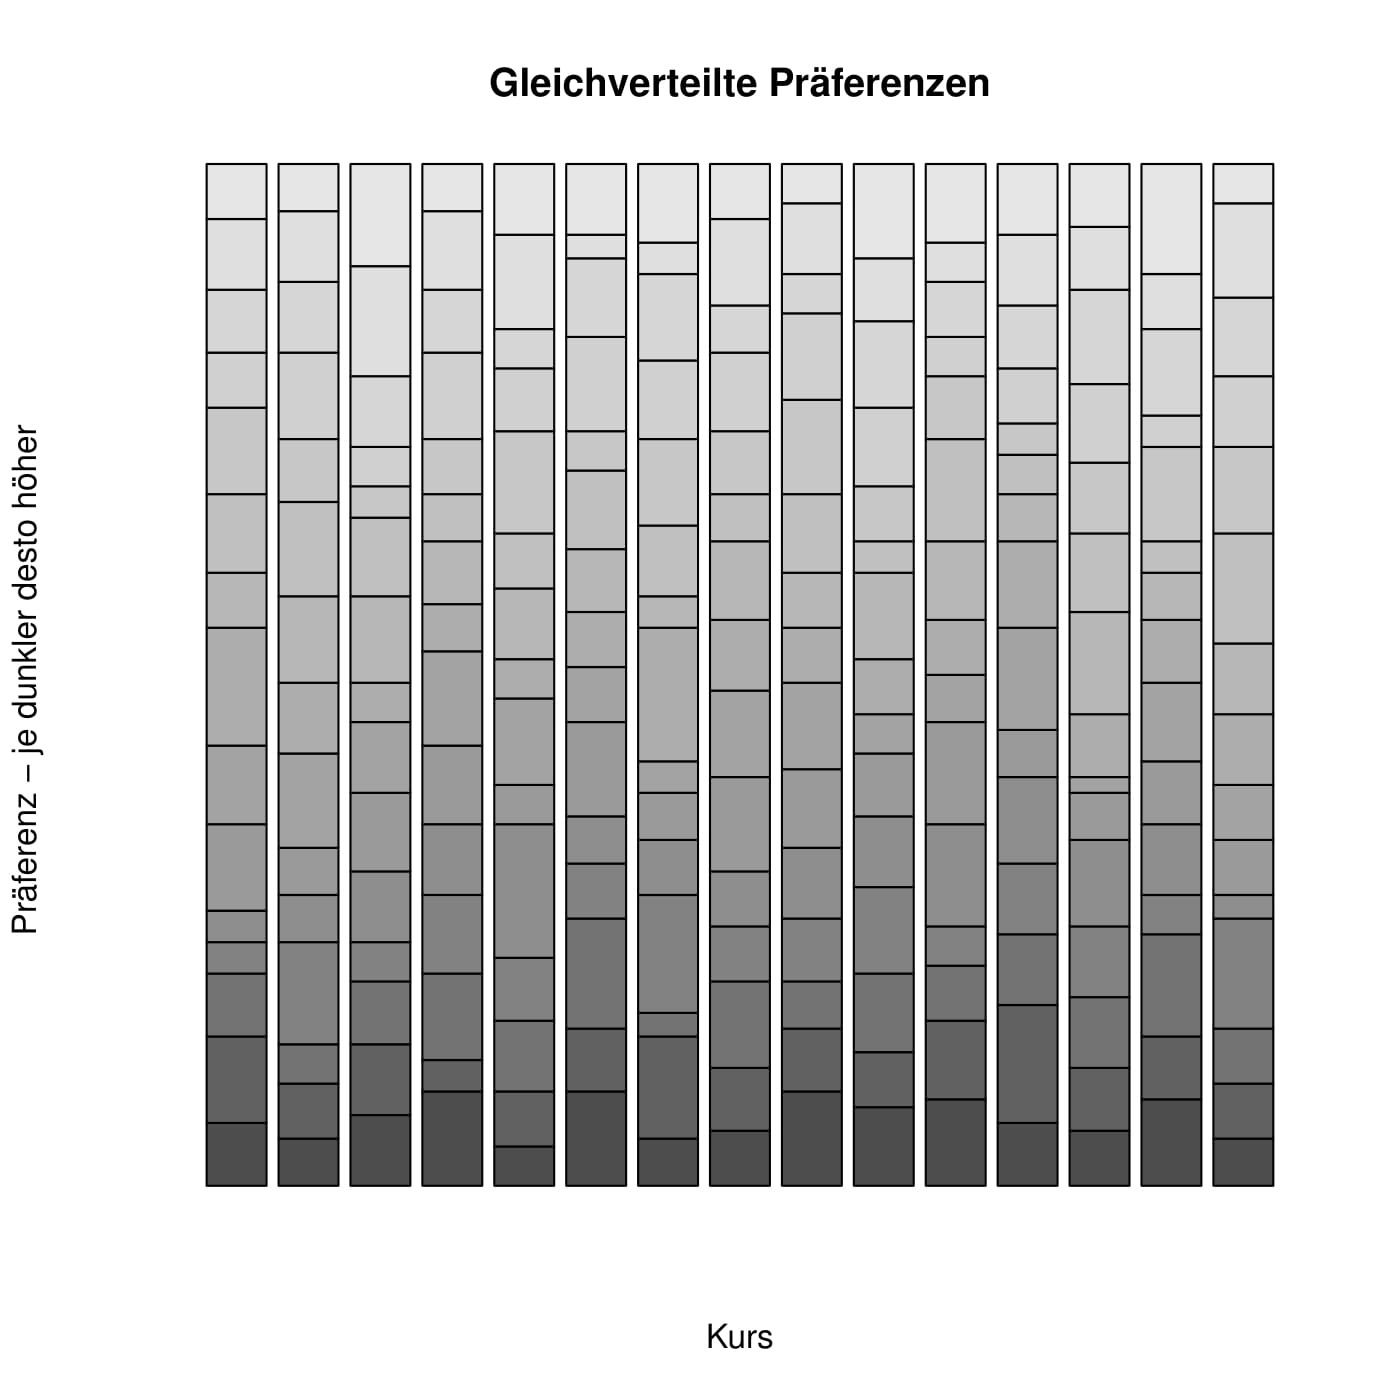
\includegraphics[width=0.7\textwidth]{./testing/images/EqualDistPreferencesDist.jpg}
				\caption{Gleichverteilte Präferenzen mit 130 Studenten auf 15 Kursen mit maximal 10 Teilnehmern pro Kurs. Die Dunkelheit stellt die Höhe der Präferenz dar}
				\label{fig:test_equal_distribution}
			\end{figure}
			Zum einen generiert dies eine gleichverteilte Präferenzenmatrix, die in Abbildung \ref{fig:test_equal_distribution} zu sehen ist.
			
			\begin{figure}
				\centering
				\begin{subfigure}{0.49\textwidth}
					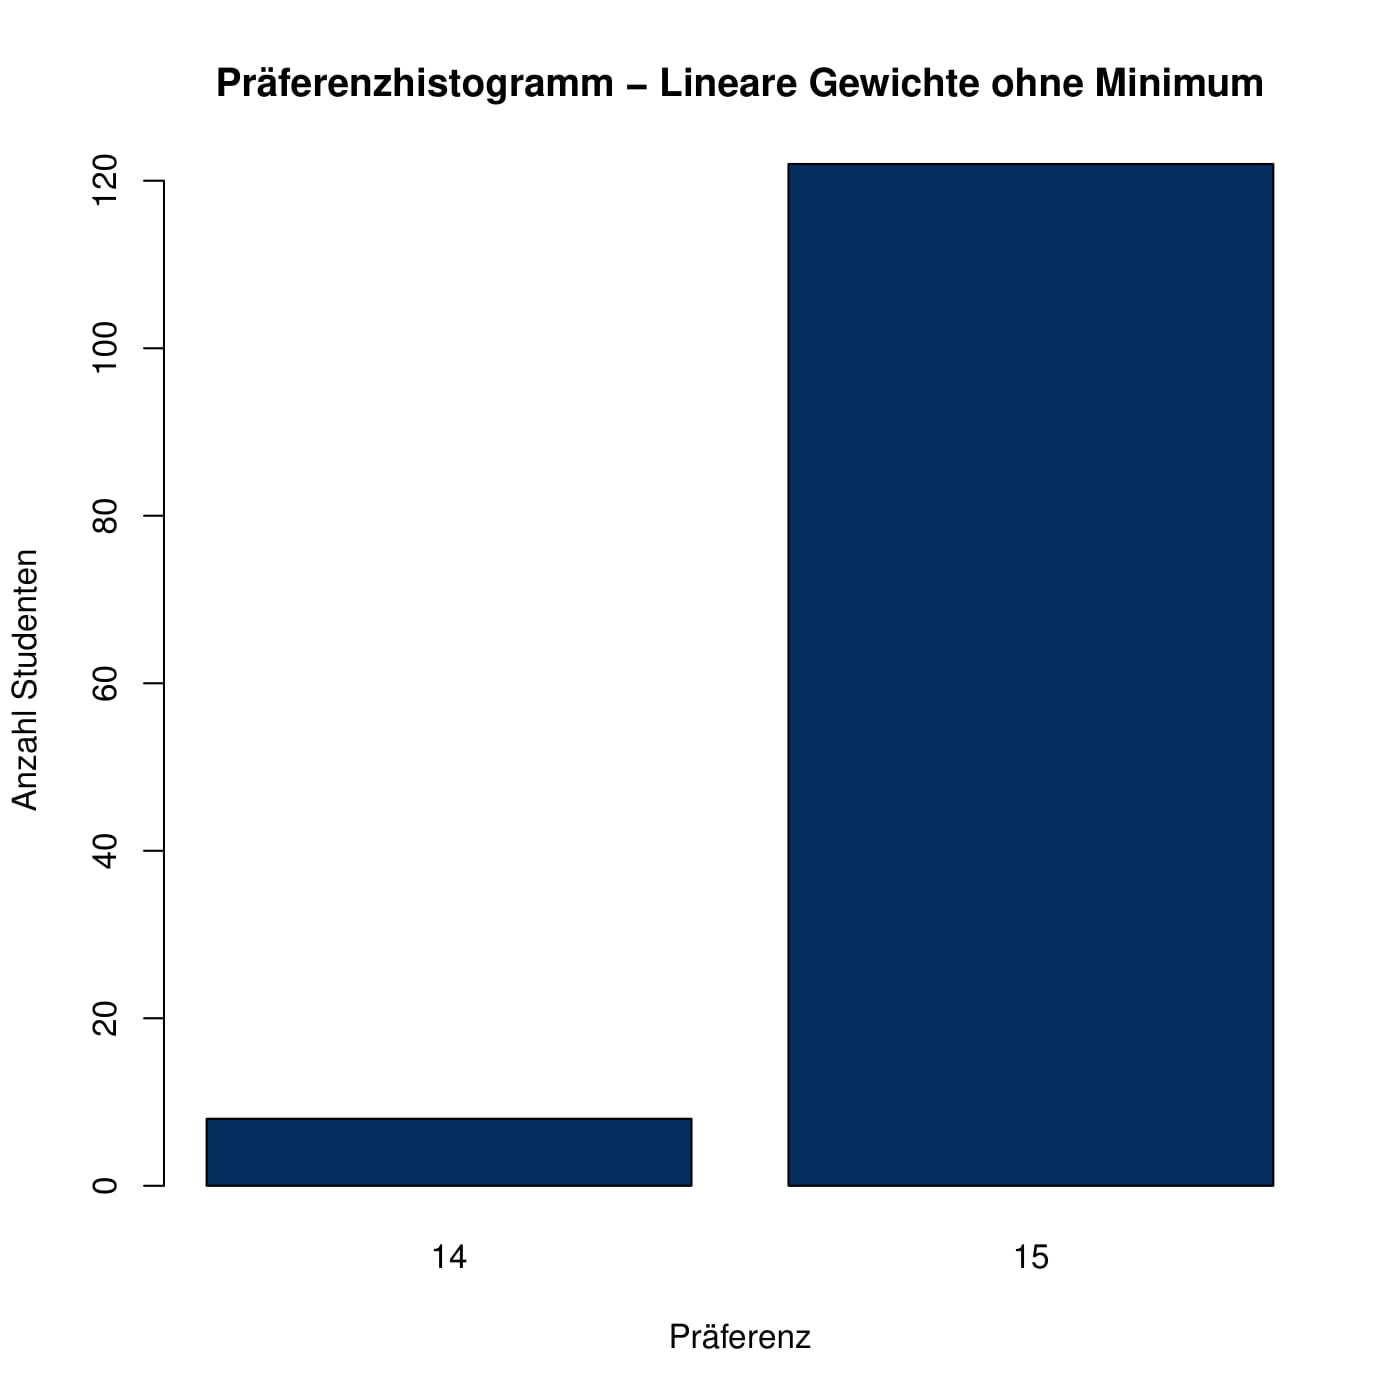
\includegraphics[width=1.0\textwidth]{./testing/images/EqualDistPreferencesHistLin.jpg}
				\end{subfigure}
				\begin{subfigure}{0.49\textwidth}
					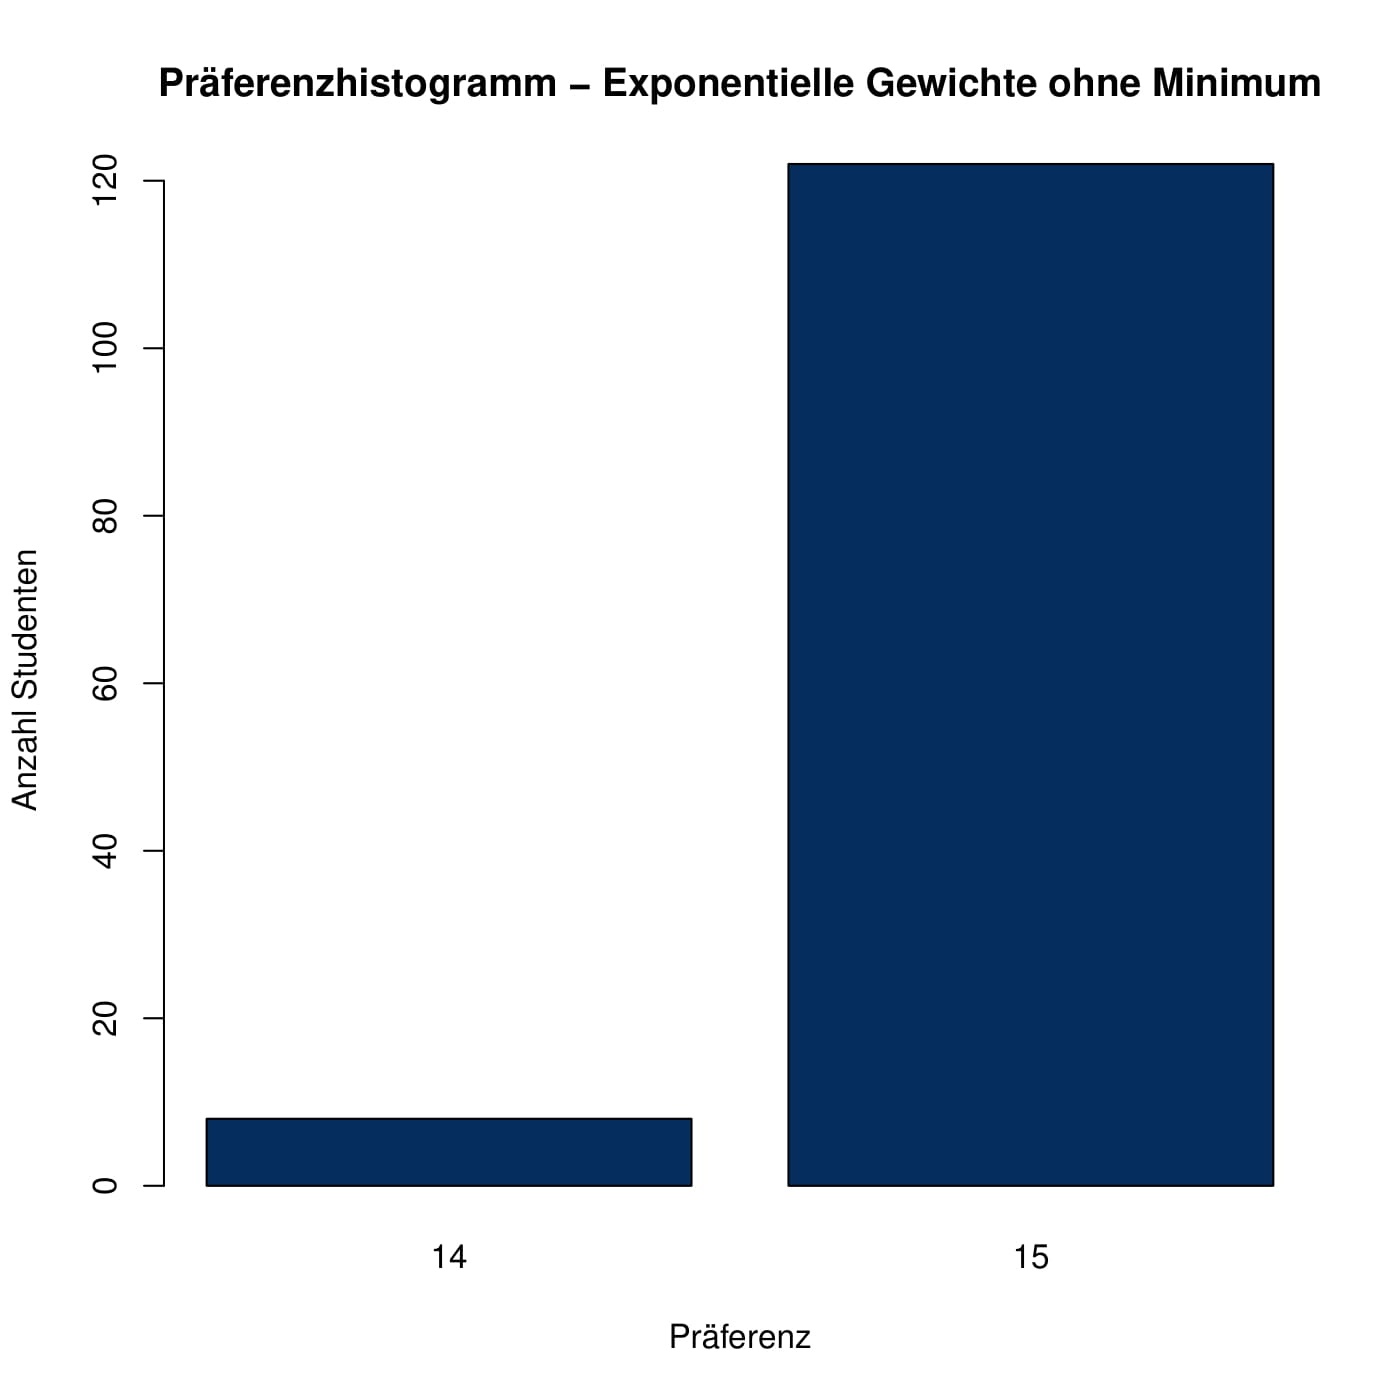
\includegraphics[width=1.0\textwidth]{./testing/images/EqualDistPreferencesHistExpo.jpg}
				\end{subfigure}
				\caption{Gegenüberstellung der Präferenzenhistogramm für lineare und exponentielle Gewichtung}
				\label{fig:test_equal_distribution_histogram}
			\end{figure}
			
			Die Verteilung ist in dem Präferenzenhistogramm in Abbildung \ref{fig:test_equal_distribution_histogram} dargestellt.
			Wie man sieht, bekommen die meisten Studenten ihre Erstwahl, das heißt den Kurs mit Präferenz 15.
			Nur sehr wenige Studenten bekommen ihre Zweitwahl, das heißt den Kurs mit Präferenz 14.\newline
			
			Der Grund hierfür ist, dass die Präferenzen auf die Kurse gleichverteilt werden.
			Das heißt, die Wahrscheinlichkeit, dass ein beliebiger Student einen beliebigen Kurs mit beliebiger Präferenz wählt, ist immer gleich.
			Allerdings ist eine gewisse Varianz in der Ziehung der Präferenzen zu beobachten.
			Daher hat jeder Kurs unterschiedlich viele Studenten pro Präferenz.
			Daher kann man davon ausgehen, dass ein paar Studenten nur ihre Zweitwahl kriegen können.\newline
		
		\subsection{Normalverteilung}
		
			\begin{figure}
				\centering
				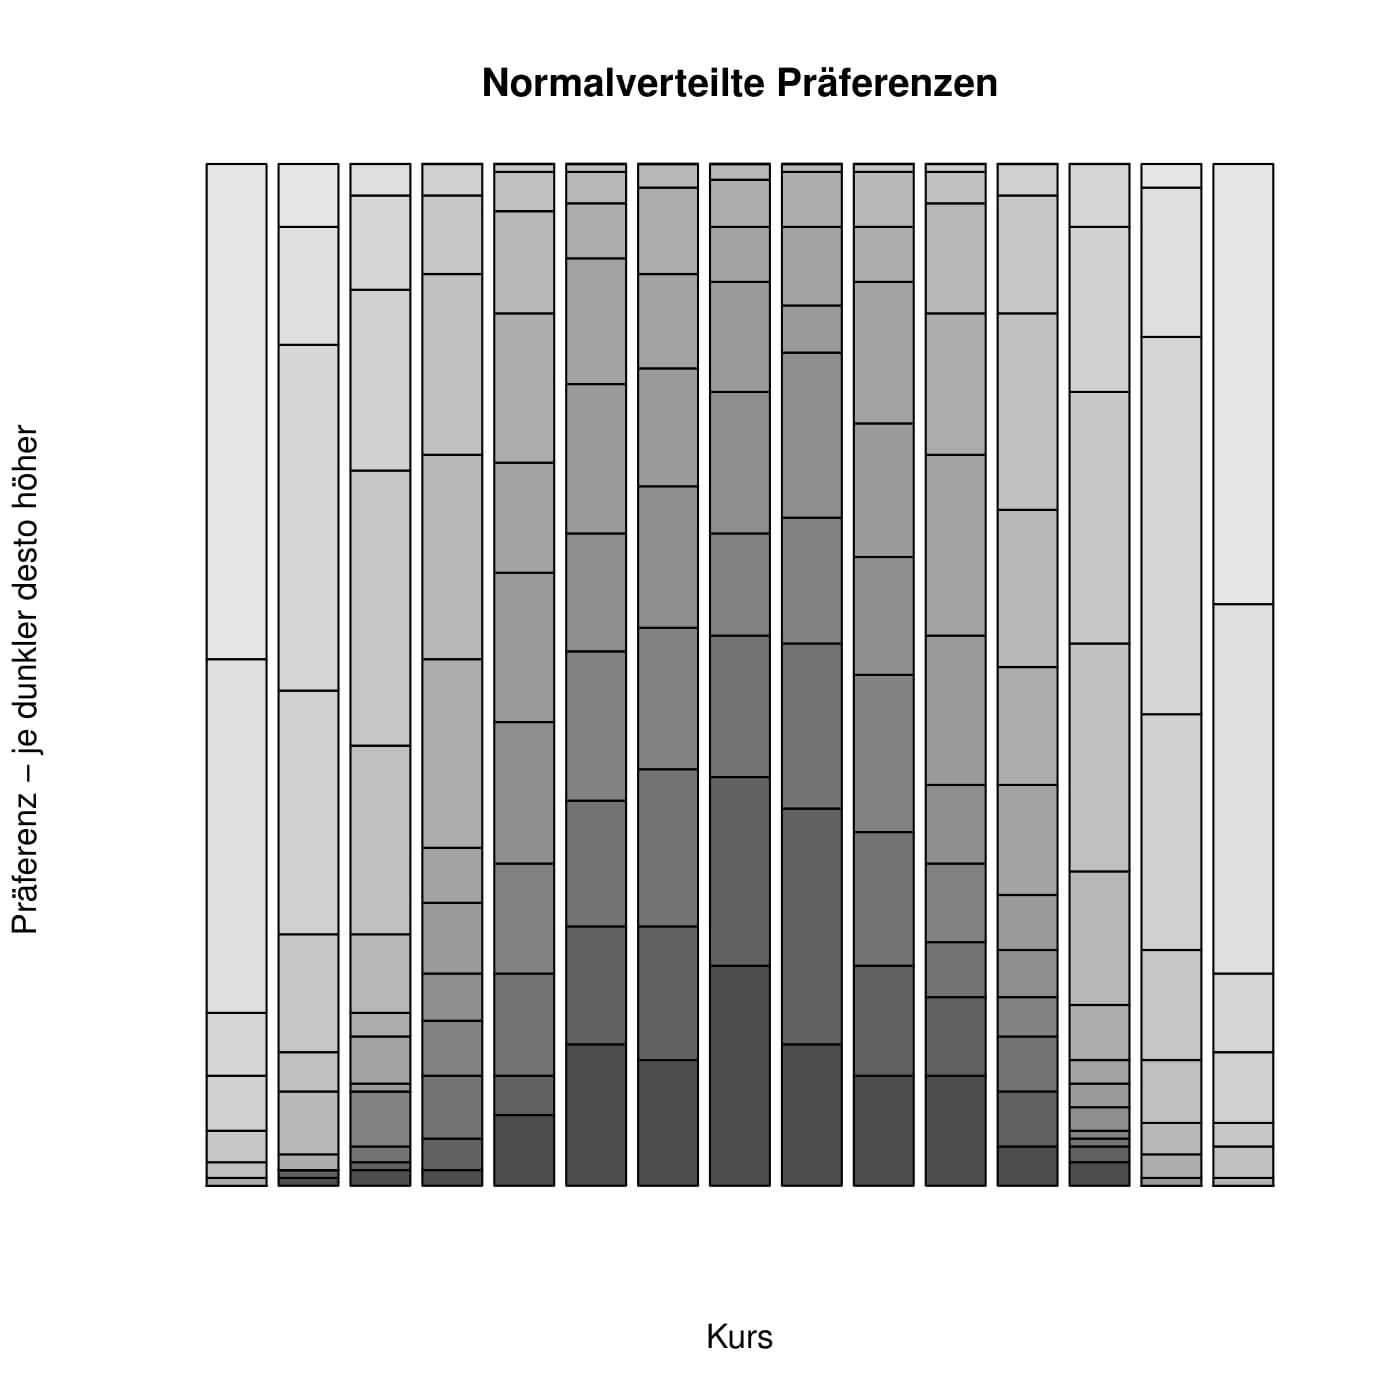
\includegraphics[width=0.7\textwidth]{./testing/images/NormalDistPreferencesDist.jpg}
				\caption{Normalverteilte Präferenzen mit 130 Studenten auf 15 Kursen mit maximal 10 Teilnehmern pro Kurs. Die Dunkelheit stellt die Höhe der Präferenz dar}
				\label{fig:test_norm_distribution}
			\end{figure}
			Weiterhin generiert das Skript eine normalverteilte Präferenzenmatrix, wie in Abbildung \ref{fig:test_norm_distribution} zu sehen ist.
			
			\begin{figure}
				\centering
				\begin{subfigure}{0.3\textwidth}
					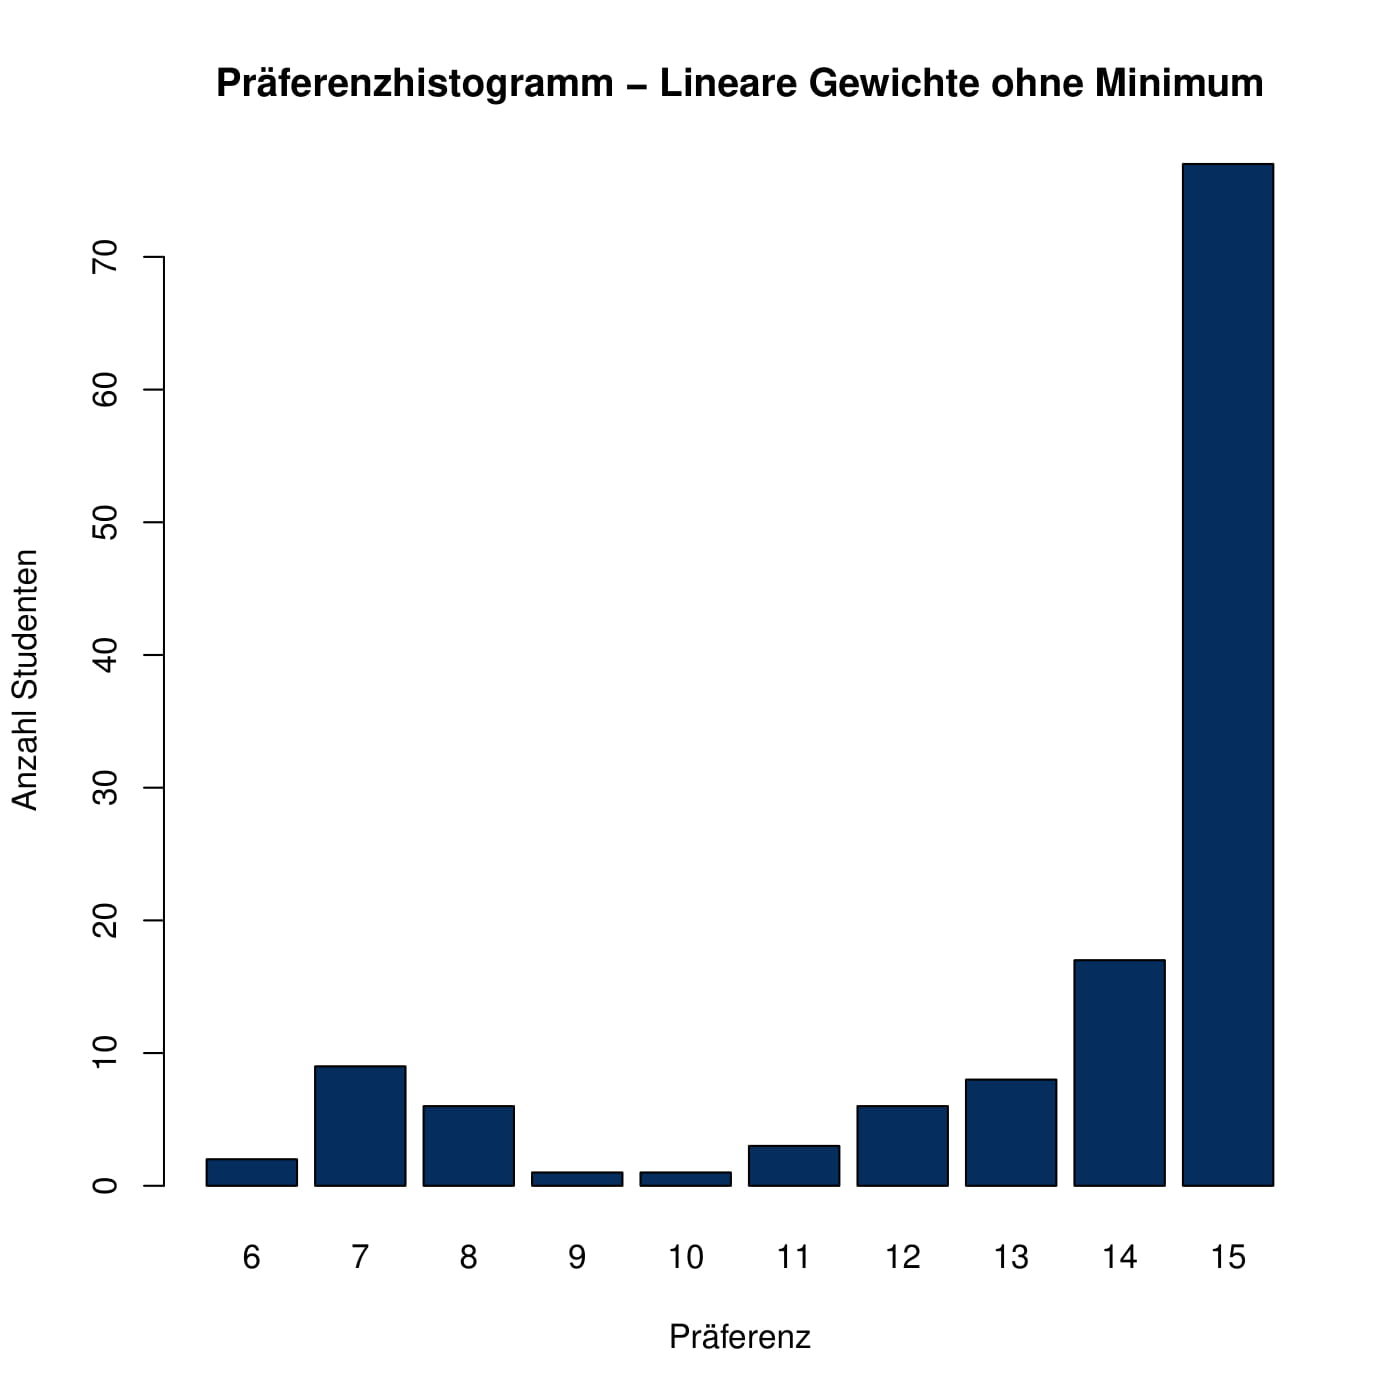
\includegraphics[width=1.0\textwidth]{./testing/images/NormalDistPreferencesHistLin.jpg}
				\end{subfigure}
				\begin{subfigure}{0.30\textwidth}
					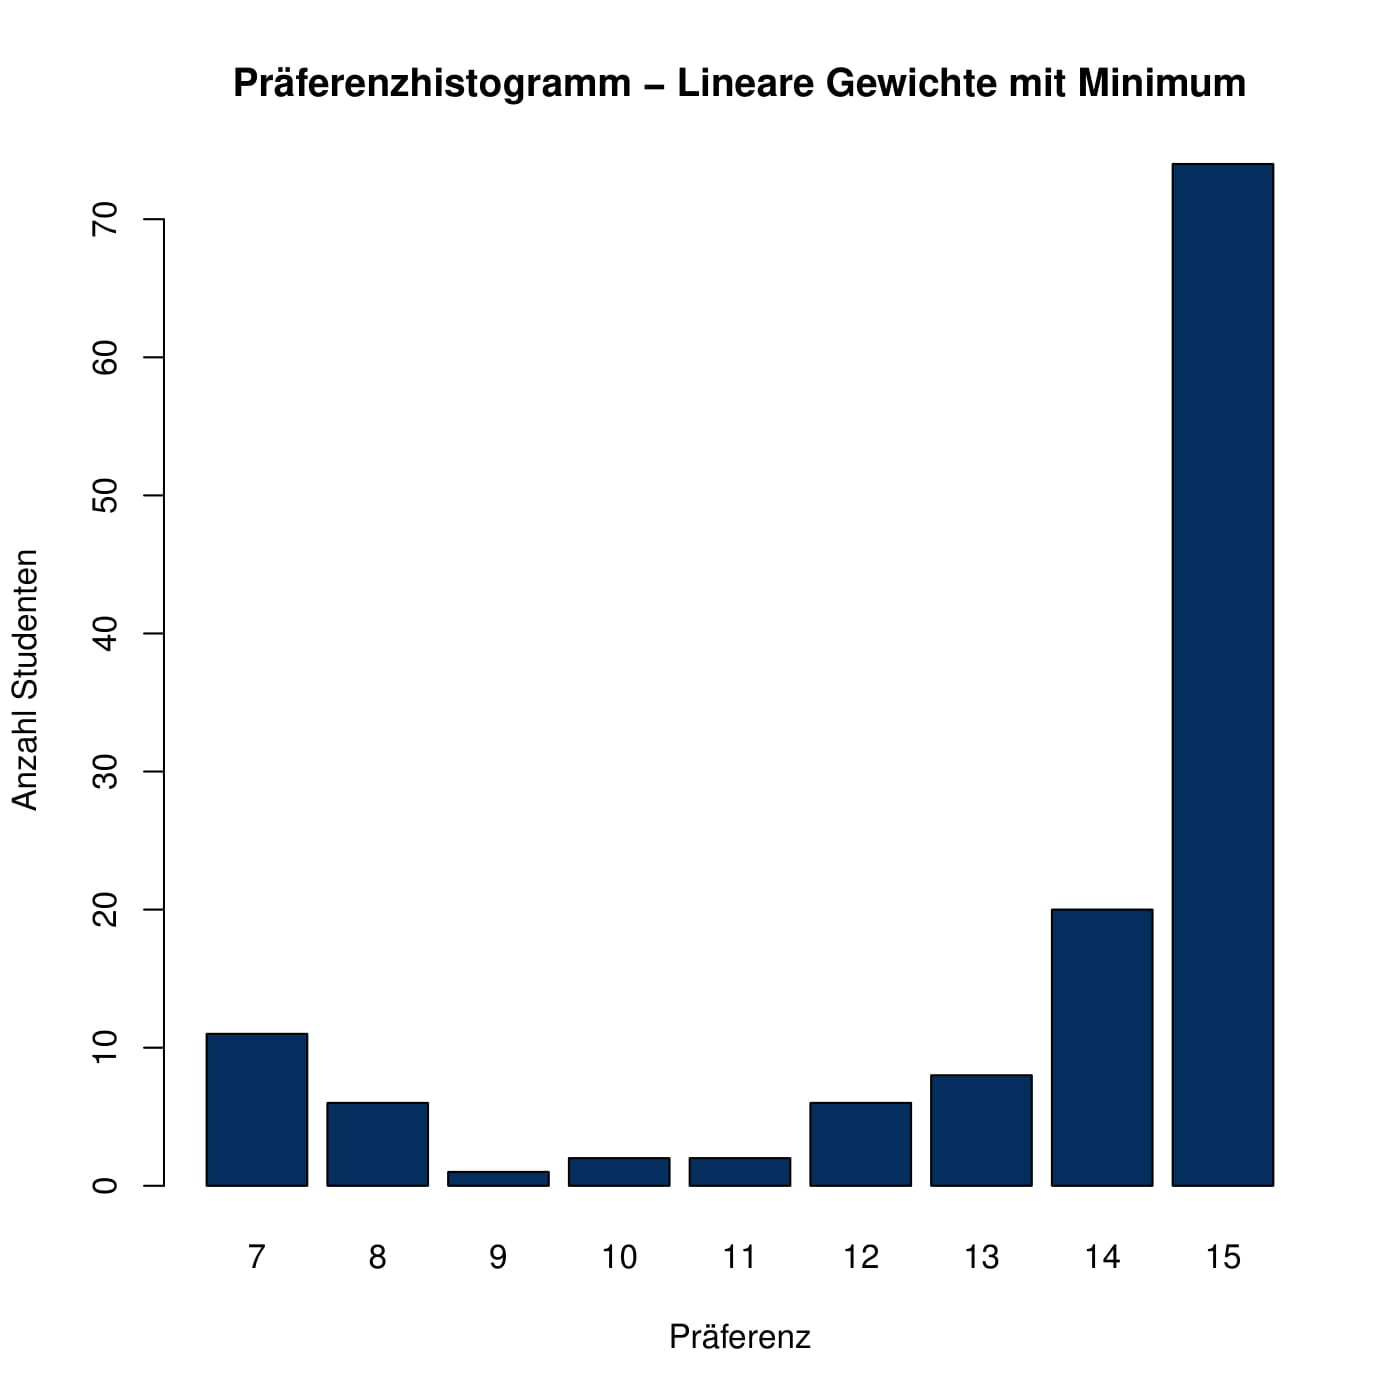
\includegraphics[width=1.0\textwidth]{./testing/images/NormalDistPreferencesHistLinMin.jpg}
				\end{subfigure}
			\begin{subfigure}{0.3\textwidth}
				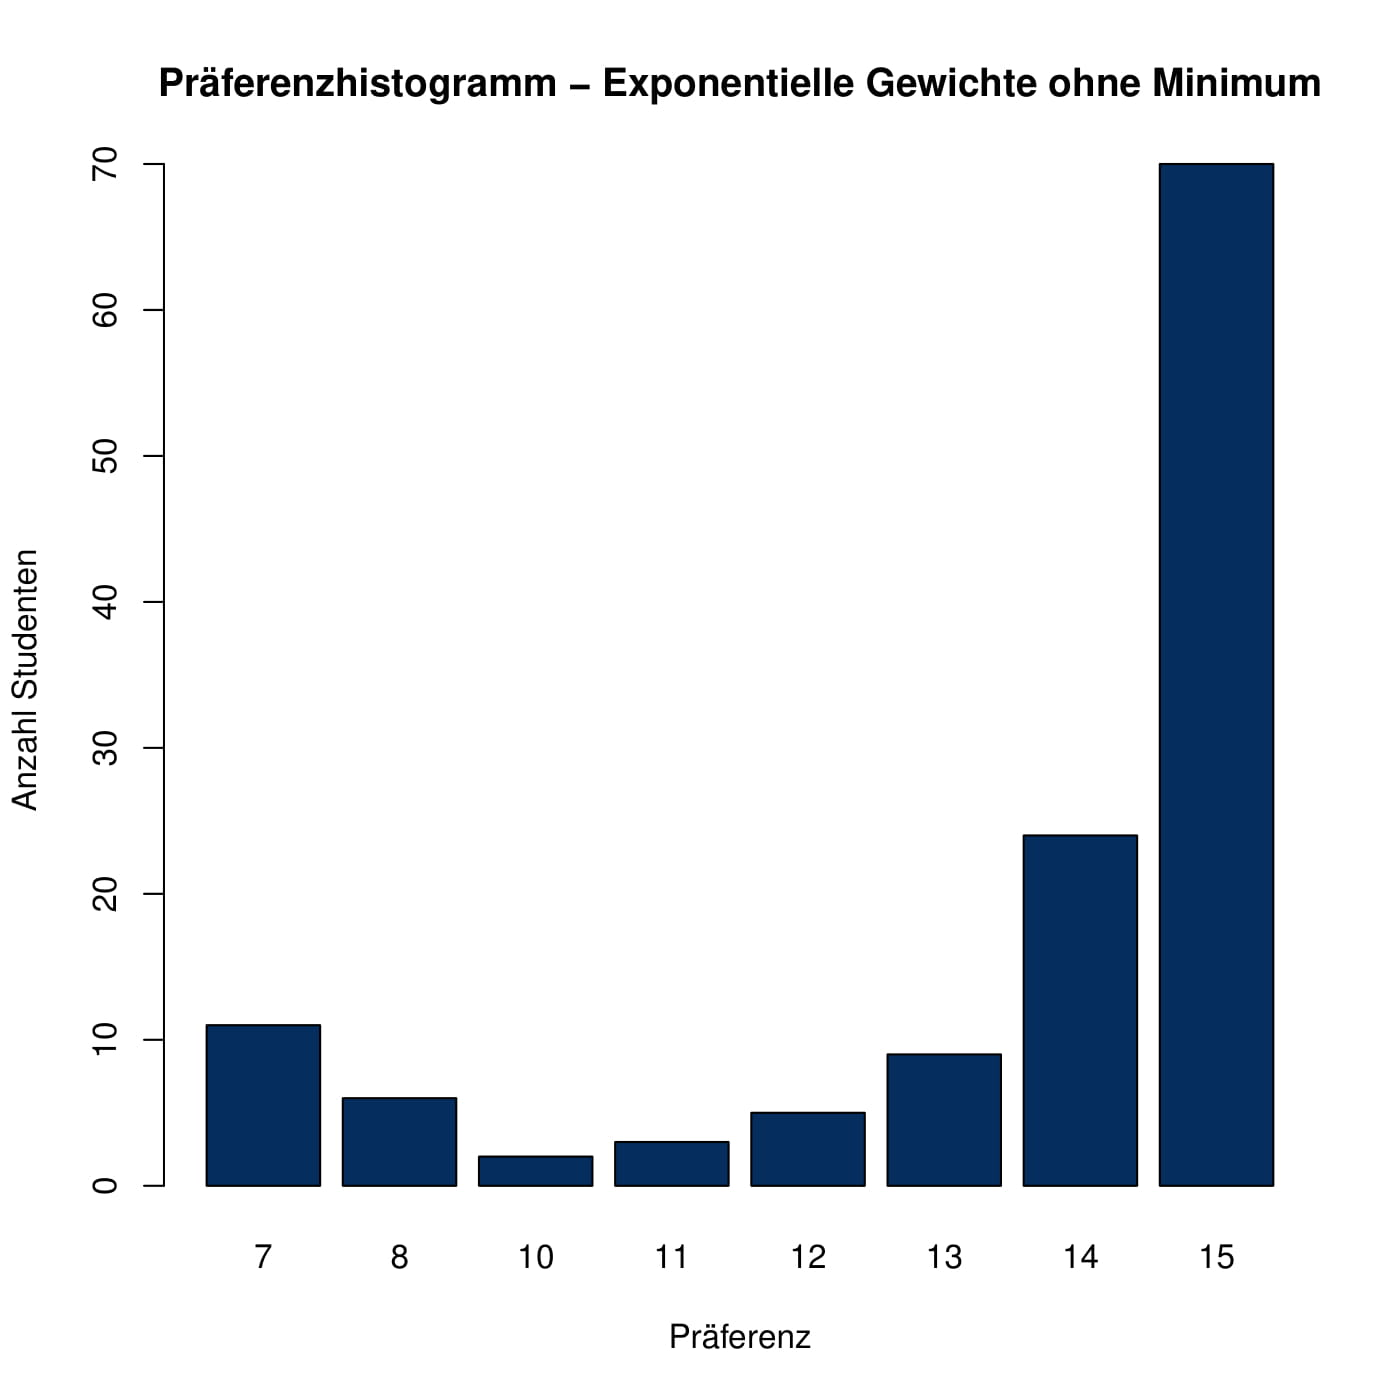
\includegraphics[width=1.0\textwidth]{./testing/images/NormalDistPreferencesHistExpo.jpg}
			\end{subfigure}
				\caption{Gegenüberstellung der Präferenzenhistogramm für lineare Gewichtung, lineare Gewichtung mit Minimum und exponentielle Gewichtung}
				\label{fig:test_norm_distribution_histogram}
			\end{figure}
		
					Die Verteilung ist in dem Präferenzenhistogramm in Abbildung \ref{fig:test_equal_distribution_histogram} dargestellt.
			Wie man sieht, bekommen in jeder der Verteilungen mehr als die Hälfte der Studenten ihre Erstwahl.
			Um die 20 Studenten bekommen allerdings nur den Kurs mit einer Präferenz kleiner 11.\newline
			
			Gut zu sehen ist, dass die Variante ''Lineare Gewichte ohne Minimum'' sich von ''Lineare Gewichte mit Minimum'' unterscheidet.
			Durch die erster Variante ist die minimale Präferenz 6, doch das Erzwingen eines festen Minimums verbessert sich diese auf 7.
			Nach den Anforderungen ist dies auch wünschenswert.
			Zuletzt ist in der Variante ''Exponentielle Gewichte ohne Minimum'' zu sehen, dass weniger Studenten ihre Erstwahl erhalten, dafür aber mehr Studenten die Präferenz 10 oder höher bekommen.\newline
			
		\subsection{Realdaten}
		
			Letztlich stellte uns der Lehrstuhl, der das Empiriepraktikum leitet, die Daten aus dem Wintersemester 2017/2018 zur Verfügung, um den neuen Algorithmus mit dem alten zu vergleichen.\newline
			
			\begin{figure}
				\centering
				\begin{tabular}{l|l|l}
					& Alter Algorithmus & Neuer Algorithmus \\
					\hline
					Mittelwert & 14.2 & 14.4 \\
					Varianz & 1,8 & 0,75 \\
					Minimale Präferenz & 7 & 12 \\
				\end{tabular}
				\caption{Vergleich des alten Algorithmus mit dem neuen Algorithmus}
				\label{tab:old_versus_new_algorithm}
			\end{figure}
		
			Wie in Abbildung \ref{tab:old_versus_new_algorithm} zu sehen ist, verbessert sich der Mittelwert, die Varianz und minimale Präferenz.
		
	\section{E-Mail Benachrichtigung}
		Zuletzt wurde die E-Mail-Benachrichtigung getestet.
		Dafür wurde der vorkonfigurierte Mailserver genutzt, der alle E-Mails abfängt.
		Dort konnten alle Mails überprüft werden.
		
		
		
		
		
		
		
		
		
		
		
		
		
		
		
		
		
		
		
		
		
		
		
		
		
